\chapter{Instrumental Variable Regression}

This chapter provides an introduction to both parametric and nonparametric instrumental variable regression.
It's goal is twofold.
Firstly, we want to introduce the subject to readers unfamiliar with it.
To make the exposition more fluid, we chose to delay the precise definition of all mathematical objects involved until Section \ref{sec: nonparametric}, which deals with the nonparametric approach.
% Until then, only knowledge of non-measure theoretic probability theory is required.
% This is sufficient to understand the motivation behind instrumental variables, as well as the most widely used tool to perform regression using them: two stages least squares.
The second goal is to precisely state the nonparametric regression problem which will be addressed in the remainder of this thesis.
Along the exposition, we will cover the basics of Two Stages Least Squares, the most widely employed IV model, and of the nonparametric approach developed by Newey and Powell in their seminal paper \cite{newey2003}.
% From that point on, we assume the reader is familiar with measure theory and linear functional analysis.
% All of the less usual objects and results we make use of will be recalled in a corresponding appendix.
% we turn our attention back to the main application being considered in this thesis: instrumental variable  regression.
% We start by characterizing the type of problem this econometric approach was developed to solve, and then present one of the most well-known and employed\unsure{Is it?} estimation procedures for conducting it: two stages least squares (2SLS).
% Nextly, we show how an IV regression problem can be formulated as a linear inverse problem and discuss the seminal nonparametric method of Newey and Powell \cite{newey2003}, followed by a more recent nonparametric approach called Kernel Instrumental Variable (KIV) \cite{singh2019}.
% We finish with an in-depth analysis of our own method\improvement{Name of the method.}, pointing out its relationship to the others, as well as its strengths and weaknesses.

\section{Endogeneity}

We start by introducing the problem of endogenous covariates.
The structural equation we consider is the following:
\begin{equation}
    \label{eq: structural equation}
    Y = \hstar ( X ) + \varepsilon
,\end{equation}
where $ X $ is a vector of explanatory variables, $ Y $ is the scalar response, $ \varepsilon $ is a zero mean noise and the function $ \hstar $ is the structural parameter we would like to estimate.
The simplest estimation method for this model specification --- and, therefore, one we would like to be able to use --- is ordinary least squares (OLS), which works by finding, within a given class of functions $ \mathcal{H} $, the element which minimizes the mean squared error:
\begin{equation}
    \label{eq: ols estimate}
    \hat{ h } = \argmin_{ h \in \mathcal{H} } \mean [ 
        ( Y - h ( X ) )^2
    ]
.\end{equation}
A reasonable and ample choice for $ \mathcal{H} $ is the set of all square-integrable functions of $ X $, that is, such that $ \mean [ h ( X )^2 ] < \infty $.
Under this choice, we recover the conditional expectation of $ Y $ given $ X $, i.e., $ \hat{ h } ( X ) = \mean [ Y \mid X ] $.
Expanding $ Y $ through (\ref{eq: structural equation}), we find that $ \hat{ h } ( X ) = \hstar ( X ) + \mean [ \varepsilon \mid X ] $.
Hence, if $ \mean [ \varepsilon \mid X ] $ is not identically null, we have introduced bias in our estimation.

This is one of the problems which appear when $ \mean [ \varepsilon \mid X ] \neq 0 $, or, more generally, when $ X $ and $ \varepsilon $ are correlated in some way.
When this happens, we say that $ X $ is \emph{endogenous}.
There are several causes for endogenous covariates, the most common of  which are \cite{wooldridge2001}:
\begin{description}
    \item[Omitted Variables] This means $ \varepsilon $ can be decomposed as $ \gstar ( W ) + \eta $, where $ \mean [ \eta \mid X, W ] = 0 $ and $ X $ and $ W $ are correlated.
        Hence, when we don't observe $ W $ and leave it to the error term, we end up estimating
        \begin{align*}
            \mean [ Y \mid X ]
            &= \hstar ( X ) + \mean [ \varepsilon \mid X ] \\
            &= \hstar ( X ) + \mean [ \gstar ( W ) + \eta \mid X ] \\
            &= \hstar ( X ) + \mean [ \gstar ( W ) \mid X ]
        \end{align*}
        which is likely different from $ \hstar ( X ) $, if $ W $ is correlated with $ X $.
        For example, if we want to regress a person's wage solely on her number of schooling years (this is $ X $), there are other variables, unaccounted for, which influence both wages and schooling, such as natural ability (this is $ W $).
        Innately skilled people may tend to be successful in school --- and, therefore, pursue higher levels of education --- as well as show higher performance in their future jobs, resulting in better wages.
        Thus, we fail to estimate $ \hstar $.
    \item[Measurement Error] If we are unable to exactly measure one of the covariates, $ X_{ k } $, and instead measure $ X_{ k }' $ subject to some stochastic error, by using $ X_{ k }' $ in our regression instead of $ X_{ k } $ we are delegating to $ \varepsilon $ some measure of the difference between $ X_{ k } $ and $ X_{ k }' $.
        Depending on how these two variables are related, we may introduce endogeneity.
        For example, $ X_{ k } $ may be a marginal tax rate, but we may only have access to an average tax rate $ X_{ k }' $.
    \item[Simultaneity] Simultaneity arises when one covariate $ X_{ k } $ is determined simultaneously with $ Y $.
        For example, if we are regressing neighborhood murder rates using the size of the local task force as a covariate, there is a simultaneity problem, since larger murder rates in a place cause a larger task force to be allocated there.
\end{description}

As we have said, bias in the estimation procedure is only one of the problems which arise when there are endogenous covariates.
It's well known that the OLS estimate for linear regression fails to be consistent if any one of the covariates is endogenous \cite{wooldridge2001}.
To overcome endogeneity a few approaches exist, but by far the one most used by empirical economic research is instrumental variable estimation \cite{wooldridge2001}.

\section{Instrumental Variables}

\begin{deff}
    \label{def: iv}
    An \emph{instrumental variable} for regression problem (\ref{eq: structural equation}) is a random variable $ Z $ such that
    \begin{enumerate}
        \item There is some influence of $ Z $ upon $ X $, that is, the marginal distribution of $ X $ is not the same as the distribution of $ X $ conditioned on $ Z $; \label{en: Z influences X}
        \item The conditional mean of $ \varepsilon $ given $ Z $ is almost surely null, i.e., $ \mean [ \varepsilon \mid Z ] = 0 $. \label{en: Z is exogenous}
    \end{enumerate}
\end{deff}

% \improvement{Causal graph, discuss strength of $ \mean[\varepsilon \mid Z] = 0$, discuss $ Z $ only influences $ Y $ through $ X $.}

The idea behind an instrumental variable is that it is exogenous \ref{en: Z is exogenous} while still influencing $ Y $ through $ X $ \ref{en: Z influences X}.
An exogenous covariate, in contrast to an endogenous one, as a variable that is determined outside of the system described by (\ref{eq: structural equation}).
% The examples ahead will clarify how instrumental variables may be chosen in practice.

Condition \ref{en: Z is exogenous} is only one of the possible meanings for the statement that $ Z $ is exogenous.
Two possible alternatives are requiring that $ Z $ be (1) independent from, or (2) uncorrelated with $ \varepsilon $.
Of course, (1) is a much more strict requirement which implies \ref{en: Z is exogenous}, while (2) is a softer condition, implied by \ref{en: Z is exogenous}.
Independence is almost always impossible to verify in real scenarios, so (1) is not a good option.
In contrast, there are situations where condition (2) is enough for ensuring good properties of IV estimators, including one we will present shortly, the linear model \cite{wooldridge2001}.
However, in order to prepare grounds for the nonparametric methods that will come later, we chose to use the definition which serves both.

Instrumental variables are also studied in the context of causal inference, where the conditions above are presented differently, in terms of causal diagrams.
In this field, instrumental variables are also required that to satisfy a third condition, phrased in terms of the causal diagram describing the relations between variables of interest \cite{hernan2020}:
\begin{enumerate}
    \setcounter{enumi}{2}
    \item All paths from $ Z $ to $ Y $ must pass through $ X $, that is, $ Z $ \emph{only} influences $ Y $ through $ X $.
\end{enumerate}
In this sense, a typical causal diagram for an IV problem is the one in Figure \ref{fig: causal diagram iv}.
\begin{figure}[t]
    \begin{center}
        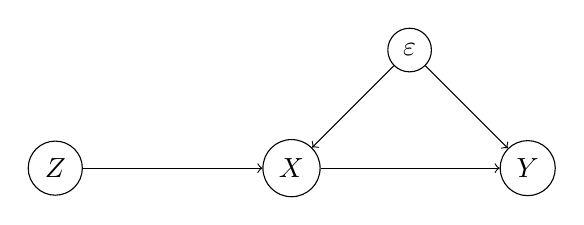
\begin{tikzpicture}[node distance=3cm]
            \node[circle,draw] at (0,0) (X) {$X$};
            \node[circle,draw,right of=X] (Y) {$Y$};
            \node[circle,draw,left of=X] (Z) {$Z$};
            \node[circle,draw,above of=X,xshift=1.5cm,yshift=-1.5cm] (eps) {$\varepsilon$};
            \draw[->] (X) -- (Y);
            \draw[->] (Z) -- (X);
            \draw[->] (eps) -- (X);
            \draw[->] (eps) -- (Y);
        \end{tikzpicture}
    \end{center}
    \caption{Causal diagram for equation (\ref{eq: structural equation}), where $ X $ is endogenous and $ Z $ is an IV.
    Source: prepared by the author.}
    \label{fig: causal diagram iv}
\end{figure}

\section{Two Stages Least Squares (2SLS)}

In this section, we restrict the structural function $ \hstar $ in (\ref{eq: structural equation}) to be affine:
\begin{equation}
    \label{}
    \hstar ( x ) = \beta_{ 0 } + \beta_{ 1 } x_{ 1 } + \cdots + \beta_{ d_{ X } } x_{ d_{ X } }
,\end{equation}
and assume to have access to a random variable $ Z $, taking values in $ \R^{ d_{ Z } } $, satisfying conditions \ref{def: iv} \ref{en: Z influences X} and \ref{en: Z is exogenous}, so that $ Z $ is a valid instrumental variable.
To ease the notation, we augment the variables $ X $ and $ Z $ to have a $ 1 $ as a first coordinate, so we may write $ \hstar ( X ) = \beta^{ \trp } X $, where $ \beta = ( \beta_{ 0 }, \dots, \beta_{ d_{ X } } ) $.
Their new dimensions are $ d_{ X }' = d_{ X } + 1 $ and $ d_{ Z }' = d_{ Z } + 1 $.
Our data is then composed of $ n $ independent joint samples $ \left\{ ( X_{ i }, Z_{ i }, Y_{ i } ) \right\}_{ i=1 }^{ n } $.
Let $ \bX \in \R^{ n \times d_{ X }' } $ and $ \bZ \in \R^{ n \times d_{ Z }' } $ be the experiment design matrices with $ 1 $'s in the first column, and let $ \bY \in \R^{ n } $ be the vector with all observations of $ Y $.
Each line of $ \bX $ and $ \bZ $ corresponds to one sample of the vectors $ X $ and $ Z $, respectively.
The idea of 2SLS is to first perform a regression of $ X $ on $ Z $ (the \emph{first stage}) and then regress $ Y $ on the fitted values $ \hat{ X } $ (the \emph{second stage}).
In what follows, we will derive this method and give some numerical examples to show its applicability.
To avoid misunderstandings during computations, we explicitly state that all vectors are regarded as \emph{column} vectors.

\subsection{Constructing the estimator}

Since we have access to an exogenous covariate, a possible idea is to use this covariate to extract from $ X $ a component which is uncorrelated with $ \varepsilon $.
The simplest way to do this is to perform the \emph{linear orthogonal projection} of $ X $ onto $ Z $, that is, to find the matrix $ P $ which minimizes the MSE:
\begin{equation*}
    P = \argmin_{ M \in \R^{ d_{ X }' \times d_{ Z }' } } \mean [ \norm{ X - M Z }^2 ] = \mathcal{L} ( M )
.\end{equation*}
A straightforward computation shows that $ \nabla \mathcal{L} ( M ) = M \mean [ Z Z^{ \trp } ] - \mean [ X Z^{ \trp } ] $.
Since $ \mathcal{L} $ is clearly convex, we may find the optimal value by setting the gradient to $ 0 $:
\begin{equation*}
    \nabla \mathcal{L} ( P ) = 0 \iff P \mean [ Z Z^{ \trp } ] = \mean [ X Z^{ \trp } ]
.\end{equation*}
We now make the hypothesis that $ \mean [ Z Z ^{ \trp } ] $ is invertible.
This means that the coordinates of $ Z $ are almost surely linearly independent, which is easy to guarantee in practice.
With that assumption, we have
\begin{equation}
    \label{eq: projection matrix formula}
    P = \mean [ X Z^{ \trp } ] \mean [ Z Z^{ \trp } ]^{ -1 }
.\end{equation}
Therefore, if we denote the fitted values $ PZ $ by $ \hat{ X } $, we may write 
\begin{equation}
    \label{eq: X on Z regression}
    X = \hat{ X } + \eta
,\end{equation}
where $ \mean [ \hat{ X } \eta^{ \trp } ] = 0 $, that is, the residual is orthogonal to the projection.

Now we go back to the structural equation, which, in the linear setting, is the following:
\begin{equation}
    \label{eq: linear structural equation}
    Y = X^{ \trp }\beta + \varepsilon
.\end{equation}
If we substitute $ X $ using equation (\ref{eq: X on Z regression}), we get
\begin{equation*}
    Y = \hat{ X }^{ \trp } \beta + \eta^{ \trp } \beta + \varepsilon
.\end{equation*}
Multiply on the left by $ \hat{ X } $ and take expectations to obtain
\begin{equation}
    \label{eq: beta is identified}
    \mean [ \hat{ X } Y ] = \mean [ \hat{ X } \hat{ X }^{ \trp } ] \beta + \mean [ \hat{ X } \eta^{ \trp } ] \beta + \mean [ \hat{ X } \varepsilon ]
.\end{equation}
We have already established that $ \mean [ \hat{ X } \eta^{ \trp } ] = 0 $.
Notice also that
\begin{equation*}
    \mean [ \hat{ X } \varepsilon ]
    = \mean [ PZ \varepsilon ]
    = \mean [ \mean [ PZ \varepsilon \mid Z ] ]
    = \mean [ PZ \mean [ \varepsilon \mid Z ] ]
    = 0
,\end{equation*}
by our definition of instrumental variable.
Equation (\ref{eq: beta is identified}) then reduces to
\begin{equation*}
    \mean [ \hat{ X } Y ] = \mean [ \hat{ X } \hat{ X }^{ \trp } ] \beta
.\end{equation*}
We would like to multiply both sides on the left by $ \mean [ \hat{ X } \hat{ X }^{ \trp } ]^{ -1 } $, but we must first check if this matrix is invertible.
Expanding we have:
\begin{equation*}
    \mean [ \hat{ X } \hat{ X }^{ \trp } ]
    = P \mean [ Z Z^{ \trp } ] P^{ \trp }
    = \mean [ X Z^{ \trp } ] \mean [ Z Z^{ \trp } ]^{ -1 } \mean [ Z X^{ \trp } ]
.\end{equation*}
Therefore, if we require the rank of the matrix $ \mean [ Z X^{ \trp } ] $ to be $ d_{ X }' $, we have invertibility of $ \mean [ \hat{ X } \hat{ X }^{ \trp } ] $.
Thus, we need to make two more assumptions: $ d_{ Z }' \geq d_{ X }' $, which is equivalent to $ d_{ Z } \geq d_{ X } $, and $ \rk \mean [ Z X^{ \trp } ] = d_{ X }' $.
The first assumption is a requirement of the second, and means that we need at least as many exogenous covariates as endogenous covariates in order to identify $ \beta $.
As for the second assumption, it is satisfied if $ X $ is sufficiently linearly related to $ Z $ \cite{wooldridge2001}. Under these conditions, we have
\begin{align}
    \label{eq: beta reduced}
    \beta
    &= \mean [ \hat{ X } \hat{ X }^{ \trp } ]^{ -1 } \mean [ \hat{ X } Y ] \\
    &= \left[
        \mean [ X Z^{ \trp } ] \mean [ Z Z^{ \trp } ]^{ -1 } \mean [ Z X^{ \trp } ]
    \right]^{ -1 }
    \mean [ X Z^{ \trp } ] \mean [ Z Z^{ \trp } ]^{ -1 } \mean [ Z Y ] \label{eq: beta expanded}
.\end{align}

The 2SLS estimator is then obtained by substituting the expectations by empirical versions, using the data in $ \bX, \bZ $ and $ \bY $.
The analogue of expression (\ref{eq: beta expanded}) would be
\begin{align}
    \label{eq: beta hat expanded}
    \begin{split}
        \hat{ \beta }
        &=
        \left[
            \left(
                \frac{ 1 }{ n } \sum_{ i=1 }^{ n } X_{ i } Z_{ i }^{ \trp }
            \right)
            \left(
                \frac{ 1 }{ n } \sum_{ i=1 }^{ n } Z_{ i } Z_{ i }^{ \trp }
            \right)^{ -1 }
            \left(
                \frac{ 1 }{ n } \sum_{ i=1 }^{ n } Z_{ i } X_{ i }^{ \trp }
            \right)
        \right]^{ -1 } \\
        &\hspace{2cm} \cdot
        \left(
            \frac{ 1 }{ n } \sum_{ i=1 }^{ n } X_{ i } Z_{ i }^{ \trp }
        \right)
        \left(
            \frac{ 1 }{ n } \sum_{ i=1 }^{ n } Z_{ i } Z_{ i }^{ \trp }
        \right)^{ -1 }
        \left(
            \frac{ 1 }{ n } \sum_{ i=1 }^{ n } Z_{ i } Y_{ i }
        \right).
    \end{split}
\end{align}        
Notice that all $ n^{ -1 } $ factors cancel out, so this may be equivalently written as
\footnote{
We remind the reader that the transpose sign changes place when writing the 2SLS estimator using data matrices, since each observation of $ X $ and $ Z $ is a \emph{line} in the corresponding matrix, not a column.
}
\begin{align*}
    \begin{split}
        \hat{ \beta }
        &= 
        \left[
            \left(
                \sum_{ i=1 }^{ n } X_{ i } Z_{ i }^{ \trp }
            \right)
            \left(
                \sum_{ i=1 }^{ n } Z_{ i } Z_{ i }^{ \trp }
            \right)^{ -1 }
            \left(
                \sum_{ i=1 }^{ n } Z_{ i } X_{ i }^{ \trp }
            \right)
        \right]^{ -1 } \\
        &\hspace{2cm} \cdot
        \left(
            \sum_{ i=1 }^{ n } X_{ i } Z_{ i }^{ \trp }
        \right)
        \left(
            \sum_{ i=1 }^{ n } Z_{ i } Z_{ i }^{ \trp }
        \right)^{ -1 }
        \left(
            \sum_{ i=1 }^{ n } Z_{ i } Y_{ i }
        \right)
    \end{split} \\
    &= \left[
        \bX^{ \trp } \bZ ( \bZ^{ \trp } \bZ )^{ -1 } \bZ^{ \trp } \bX
    \right]^{ -1 }
    \bX^{ \trp } \bZ ( \bZ^{ \trp } \bZ )^{ -1 } \bZ^{ \trp } \bY
.\end{align*}
Letting $ \hat{ \bX } $ denote $ \bX^{ \trp } \bZ ( \bZ^{ \trp } \bZ )^{ -1 } \bZ^{ \trp } $, we have
\begin{equation*}
    \hat{ \beta } = \left( \hat{ \bX } \hat{ \bX }^{ \trp } \right)^{ -1 } \hat{ \bX } \bY 
,\end{equation*}
which is the empirical analogue of equation (\ref{eq: beta reduced}).
This final form makes it clear that the estimator $ \hat{ \beta } $ is obtained by first performing one linear regression of $ \bX $ onto $ \bZ $, and then taking the fitted values $ \hat{ \bX } $ and linearly regressing $ \bY $ on them.

Using equation (\ref{eq: beta hat expanded}), together with the Law of Large Numbers and Slutsky's Theorem, one may prove the consistency of $ \hat{ \beta } $.
Similar inspection allows one to establish asymptotic normality.
For further theoretical properties of the 2SLS estimator, we refer the reader to \cite[Chapter~5]{wooldridge2001}, this section's main reference.

\subsection{Numerical examples}

We now provide numerical examples to strengthen our intuition about the differences between OLS and 2SLS.
We present two scenarios with the same joint distribution for $ X $ and $ Z $, in which both are one dimensional.
The scenarios also share the same structural function, which we set to be $ \hstar ( x ) = \beta_{ 0 } + \beta_{ 1 }x $, with $ \beta_{ 0 } = 0.3 $ and $ \beta_{ 1 } = 0.7 $.
The difference between both experiments is the distribution of $ \varepsilon $, which is mildly codependent with that of $ X $ in the first experiment, and strongly codependent in the second.

The data generating process we use for $ X $ and $ Z $ is the following:
\begin{align*}
    \delta_{ i } &\iid \mathcal{N} ( 0, 1 ), \quad i = 1, 2; \\
    Z &= \Phi ( \delta_{ 1 } ); \\
    X &= \Phi ( \rho \delta_{ 1 } + \sqrt{ 1 - \rho^2 } \delta_{ 2 } )
,\end{align*}
where $ \Phi $ is the cumulative distribution function of the standard normal and $ \rho \in ( 0, 1 ) $ is fixed at $ 0.8 $.
For the first scenario, we generate $ \varepsilon $ as follows:
\begin{align*}
    \delta_{ 3 } &\sim \mathcal{N} ( 0, 1 ), \quad \delta_{ 3 } \indep ( \delta_{ 1 }, \delta_{ 2 } ); \\
    \varepsilon &= \sigma \cdot ( \eta \delta_{ 2 } + \sqrt{ 1 - \eta^2 } \delta_{ 3 } )
,\end{align*}
where $ \sigma > 0 $ and $ \eta \in ( 0, 1 ) $ are set to be $ 0.1 $ and $ 0.6 $, respectively.
For the second scenario, we introduce more interdependence between $ X $ and $ \varepsilon $:
\begin{align*}
    \varepsilon = \sigma \cdot \left(
        \left[ \eta \delta_{ 2 } + \sqrt{ 1 - \eta^2 } \delta_{ 3 } \right]
        + C_{ b } ( \delta_{ 2 } - b )^{ + } - C_{ a } ( \delta_{ 2 } - a )^{ - }
    \right)
.\end{align*}
Here, $ \sigma $ and $ \eta $ have the same values as before.
The additional terms are $ C_{ b } = 6, b = 0.7, C_{ a } = 2 $ and $ a = 0.3 $.
Finally, in both formulations we have $ Y = \hstar ( x ) + \varepsilon $.

The results of the experiments are in Figure \ref{fig: 2sls vs ols}.
We can see that in both of them the 2SLS estimate is closer to the true values of $ \beta_{ 0 } $ and $ \beta_{ 1 } $ than the OLS estimate.
As expected, the OLS estimate does not take endogeneity into account and, therefore, incorporates some bias into the final estimates.
This effect worsens as the endogeneity becomes stronger.
An important observation, which is not visible in the figure, is that, as the number of observations grows, the OLS estimate drifts further from the true values, while the 2SLS estimate becomes closer to them.

\begin{figure}[htb]
    \begin{center}
        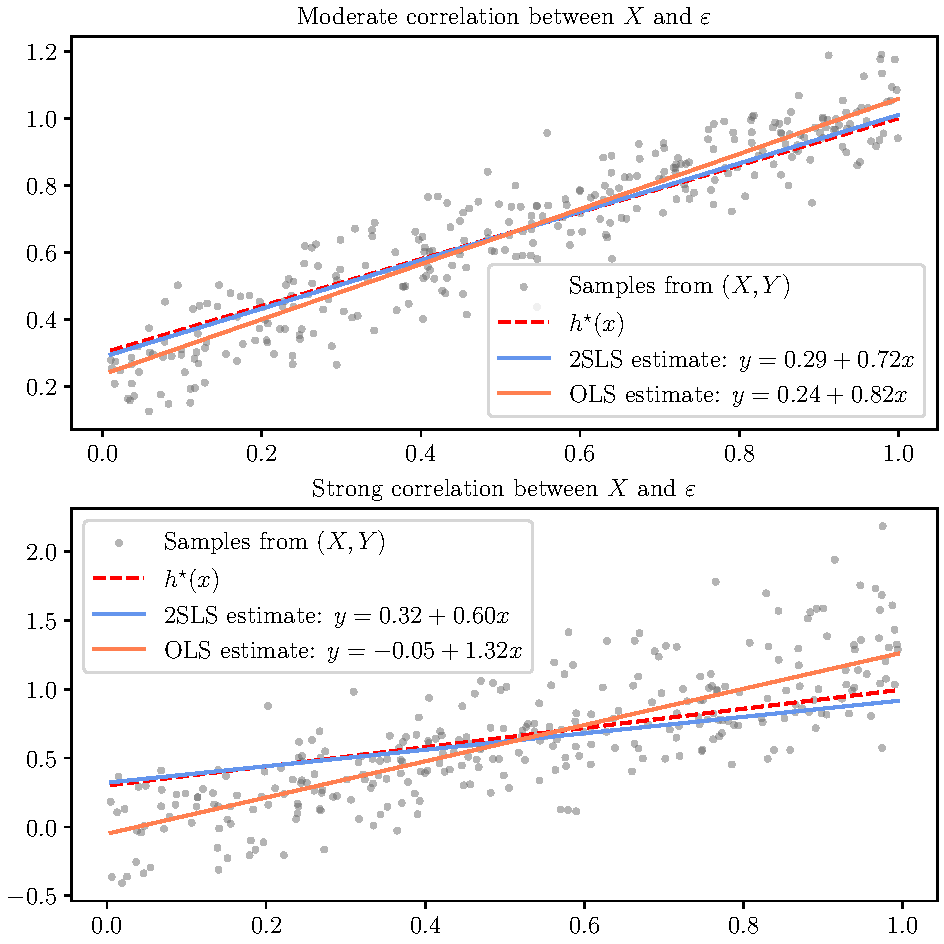
\includegraphics{tsls_examples.pdf}
    \end{center}
    \caption{Comparison between OLS and 2SLS under two different levels of endogeneity.}
    \label{fig: 2sls vs ols}
\end{figure}

\section{Nonparametric Instrumental Variable Regression}
\label{sec: nonparametric}

In nonparametric regression, we do not specify \emph{a priori} a finite dimensional parametric form for the structural function (such as restricting it to be affine), and so we allow our search space to potentially be infinite dimensional.
However, in doing this, we must still precisely define the infinite dimensional space where the solution will be searched for.
Hence, we start by precisely defining the nonparametric regression problem given by (\ref{eq: structural equation})

\subsection{Problem specification}
\label{sec: problem specification}

Let $ ( \Omega, \mathcal{A}, \prob ) $ be the underlying probability space.
Assume that $ X : ( \Omega, \mathcal{A} ) \to ( \R^{ d_{ X } }, \mathcal{B} ( \R^{ d_{ X } } ) ) $ and $ \varepsilon : ( \Omega, \mathcal{A} ) \to ( \R, \mathcal{B} ( \R ) ) $ are measurable\footnotemark~and, furthermore, that $ \varepsilon \in L^{ 1 } ( \Omega, \mathcal{A}, \prob ) $ with $ \mean [ \varepsilon ] = 0 $.
\footnotetext{We denote by $ \mathcal{B} ( \R^{ k } ) $ the Borel $ \sigma $-algebra in $ \R^{ k } $.}
We also assume that $ \mean [ \varepsilon \mid X ] $ is \emph{not} almost surely null and, hence, $ X $ is endogenous.
Denote by $ \prob_{ X } $ the distribution of the random variable\footnote{We use the term ``random variable'' when referring to scalar or vector valued measurable functions defined on $ ( \Omega, \mathcal{A} ) $.} $ X $, that is, the pushforward measure $ \prob \circ X^{ -1 } $ defined on $ \mathcal{B} ( \R^{ d_{ X } } ) $.
We write $ L^{ 2 } ( X ) $ as a shorthand for the space $ L^2 ( \R^{ d_{ X } }, \mathcal{B} ( \R^{ d_{ X } } ), \prob_{ X } ) $ of real and square integrable (equivalence classes of) measurable functions defined on the measure space $ ( \R^{ d_{ X } }, \mathcal{B} ( \R^{ d_{ X } } ), \prob_{ X } ) $.
It's important to recall that the inner product and norm in $ L^{ 2 } ( X ) $ are given by $ \dotprod{ h, g }_{ L^{ 2 } ( X ) } = \mean [ h ( X ) g ( X ) ] $ and $ \norm{ h }_{ L^{ 2 } ( X ) }^2 = \dotprod{ h, h }_{ L^{ 2 } ( X ) } = \mean [ h ( X )^2 ] $.

We assume there exists $ \hstar \in L^{ 2 } ( X ) $ such that (\ref{eq: structural equation}) holds, that is, $ Y = \hstar ( X ) + \varepsilon $.
Finally, we assume there exists a random variable $ Z : ( \Omega, \mathcal{A} ) \to ( \R^{ d_{ Z } }, \mathcal{B} ( \R^{ d_{ Z } } ) ) $ such that $ Z $ qualifies as an instrumental variable, i.e., $ Z $ satisfies conditions \ref{def: iv} \ref{en: Z influences X} and \ref{en: Z is exogenous}.
We define $ \prob_{ Z } $ and $ L^{ 2 } ( Z ) $ in an manner analogous to $ \prob_{ X } $ and $ L^{ 2 } ( X ) $.
Our goal is to estimate $ \hstar $ based on i.i.d. samples from the joint distribution of $ X, Z $ and $ Y $.

\subsection{Identification}

An important question to ask after specifying the problem is whether the function $ \hstar $ is identified.
The answer is negative without further assumptions, which will be presented in this subsection.
This discussion was inspired on \cite[Section~2]{newey2003}.

Suppose there exists $ \delta \in L^{ 2 } ( X ) $ such that $ \delta \neq 0 $, but $ \mean [ \delta ( X ) \mid Z ] = 0 $.
Without loss of generality, we can assume\footnotemark~ $ \delta ( X ) \neq \mean [ \varepsilon \mid X ] $.
\footnotetext{If it happens to be the case that $ \mean \left[ \mean [ \varepsilon \mid X ] \mid Z \right] $ = 0 (which is \emph{not} implied by our assumptions so far), we can simply take $ \delta ( X ) = \lambda \mean [ \varepsilon \mid X ] $, for some $ \lambda \in \R \setminus \left\{ 0, 1 \right\} $.
Since, by hypothesis, $ \mean [ \varepsilon \mid X ] \neq 0 $, this satisfies our requirements and is different from $ \mean [ \varepsilon \mid X ] $.}
Defining $ g \defeq \hstar + \delta $ and $ \eta \defeq \varepsilon - \delta ( X ) $, we have
\begin{equation*}
    Y = g ( X ) + \eta
,\end{equation*}
where $ \mean [ \eta \mid Z ] = 0 $ and $ \mean [ \eta \mid X ] \neq 0 $.
Hence, $ g \neq \hstar $ but they are indistinguishable from the data generating process' perspective.
Reciprocally, suppose that the only member of $ L^{ 2 } ( X ) $ which has null mean conditioned on $ Z $ is the null function.
Then, given $ g \in L^{ 2 } ( X ) $ such that
\begin{equation*}
    Y = g ( X ) + \eta
\end{equation*}
with $ \mean [ \eta \mid Z ] = 0 $, we have
\begin{equation*}
    0 = ( g - \hstar ) ( X ) + \eta - \varepsilon
.\end{equation*}
Conditioning on $ Z $, we get
\begin{equation*}
    \mean [ ( g - \hstar ) ( X ) \mid Z ] = 0
,\end{equation*}
which, by assumption, implies $ \hstar = g $.

Therefore, a necessary and sufficient condition for identification of our regression problem is the following:
\begin{assump*}[Identification]
    If $ \delta \in L^{ 2 } ( X ) $ satisfies $ \mean [ \delta ( X ) \mid Z ] = 0 $, then $ \delta = 0 $.
\end{assump*}

This condition has an interpretation in terms of the conditional expectation operator, which will be a key object in the construction of our estimator for $ \hstar $.
Let $ h \in L^{ 2 } ( X ) $.
Notice that, by Jensen's inequality,
\begin{equation}
    \label{eq: P is bounded}
    \mean [ ( \mean [ h ( X ) \mid Z ] )^2 ]
    \leq \mean [ \mean [ h ( X )^2 \mid Z ] ]
    = \mean [ h ( X )^2 ]
    < +\infty
.\end{equation}
Furthermore, since $ \mean [ h ( X ) \mid Z ] $ is a $ \sigma ( Z ) $-measurable\footnote{We denote by $ \sigma ( Z ) $ the smallest $ \sigma $-algebra in $ \Omega $ with respect to which $ Z $ is measurable.} random variable, by the Doob-Dynkin Lemma there exists a measurable function $ f_{ h } : ( \R^{ d_{ Z } }, \mathcal{B} ( \R^{ d_{ Z } } ) ) \to ( \R, \mathcal{B} ( \R ) ) $ such that
\begin{equation*}
    \mean [ h ( X ) \mid Z ] = f_{ h } ( Z )
.\end{equation*}
Under these conditions, we write $ \mean [ h ( X ) \mid Z = z ] $ for $ f_{ h } ( z ) $.
The computation in (\ref{eq: P is bounded}) shows that $ f_{ h } \in L^2 ( Z ) $ for every $ h \in L^2 ( X ) $.
Therefore, we can define the operator $ \meanop : L^2 ( X ) \to L^2 ( Z ) $ given by $ \meanop [ h ] = f_{ h } = \mean [ h ( X ) \mid Z = \cdot ] $.
This operator, called the \emph{conditional expectation operator}, is clearly linear and, again by (\ref{eq: P is bounded}), also bounded, satisfying $ \norm{ \meanop }_{ \op } \leq 1 $.
The identification assumption thus amounts to saying that the kernel of $ \meanop $ is trivial, i.e., $ \meanop $ is injective.

It is hard to quantify how restrictive this condition is for arbitrary $ X $ and $ Z $, so we analyze it in a more familiar setting, the exponential family.
We will use a classic completeness result for statistics in this family of distributions to reformulate the identification assumption in terms of more familiar objects.
We first define completeness:
\begin{deff}
    \cite{lehmann59} We say that a family $ \mathscr{P} $ of probability distributions on a measurable space $ ( E, \mathcal{E} ) $ is \emph{complete} if
    \begin{equation*}
        \int_{ E } f ( x ) \ P ( \ddrm x ) = 0 \quad \text{for all} \quad P \in \mathscr{P}
    \end{equation*}
    implies $ f ( x ) = 0 $ $ \mathscr{P} $-a.e\footnote{We say that a statement $ Q ( x ) $ is true $ \mathscr{P} $-a.e. if there exists a set $ N \in \mathcal{E} $ such that $ Q ( x ) $ is true for $ x \in E \setminus N $ and $ P ( N ) = 0 $ for all $ P \in \mathscr{P} $.}.
\end{deff}
Then, a remarkable fact about the exponential family is the completeness of the natural statistics under a mild condition on the set of parameters:
\begin{thm}
    \label{thm: completeness of exp family}
    \cite{lehmann59} Let $ \Xi $ be a subset of an Euclidian space with nonempty interior.
    Let $ X $ be a random vector with distribution $ P^{ \theta } $ parametrized by $ \theta \in \Xi $ in the following manner:
    \begin{equation*}
        P^{ \theta } ( \ddrm x ) = C ( \theta ) \exp \left\{ \sum_{ i=1 }^{ s } \theta_{ i } T_{ i } ( x ) \right\} \mu ( \ddrm x )
    ,\end{equation*}
    where $ \mu $ is the underlying measure.
    Then, the family $ \mathscr{P}_{ T } $, formed by the distributions of the random vector $ T ( X ) = ( T_{ 1 } ( X ), \dots, T_{ s } ( X ) ) $ as $ \theta $ ranges through $ \Xi $, is complete.
\end{thm}

Using this result and under suitable hypotheses, we can reformulate the identification condition.
\begin{thm}
    For $ z \in \R^{ d_{ z } } $, let $ \probq_{ z } : \mathcal{B} ( \R^{ d_{ X } } ) \to [0, 1] $ denote the conditional distribution of $ X $ given $ Z = z $.
    Assume there exists $ U \in \borel ( R^{ d_{ Z } } ) $ such that $ \prob_{ Z } ( U ) = 1 $ and for all $ z \in U $ we have
    \begin{equation*}
        \probq_{ z } ( \ddrm x ) = C ( z ) \exp ( \alpha ( z )^{ \trp } T ( x ) ) \; \mu ( \ddrm x )
    \end{equation*}
    for an underlying measure $ \mu $ on $ \borel ( \R^{ d_{ X } } ) $ and some functions $ \alpha : \R^{ d_{ z } } \to \R^{ s } $ and $ T : \R^{ d_{ x } } \to \R^{ s } $.
    Assume that $ T $ is injective and that the image of $ \alpha $ restricted to $ U $ contains an open set.
    Then, $ \hstar $ is identified.
\end{thm}
\begin{proof}
    Taking $ \Xi = \alpha ( U ) $ and $ \theta = \alpha ( z ) $, we see that the hypotheses of Theorem \ref{thm: completeness of exp family} are satisfied and, hence,
    \begin{equation*}
        \mathscr{P} \defeq \left\{ \probq_{ z } \circ T^{ -1 } : z \in U \right\}
    \end{equation*}
    is a complete family of probability distributions.
    Let $ h \in L^2 ( X ) $ be such that $ \meanop [ h ] = 0 $, i.e., $ \mean [ h ( X ) \mid Z ] = 0 $ $ \prob_{ Z } $-a.s.
    This means that the function
    \begin{equation*}
        z \longmapsto \int_{ \R^{ d_{ x } } } h ( x ) \ \probq_{ z } ( \ddrm x )
    \end{equation*}
    is null $ \prob_{ Z } $-a.s.
    Without loss of generality, we may assume that its null on $ U $.
    But notice that, since $ T $ is injective, we can rewrite this integral as
    \begin{align*}
        0 = \int_{ \R^{ d_{ x } } } h ( x ) \ \probq_{ z } ( \ddrm x )
        &= \int_{ \R^{ d_{ x } } } ( h \circ T^{ -1 } ) ( T ( x ) ) \ \probq_{ z } ( \ddrm x ) \\
        &= \int_{ \R^{ s } } ( h \circ T^{ -1 } ) ( t )  \ ( \probq_{ z } \circ T^{ -1 } ) ( \ddrm t )
    \end{align*}
    for all $ z \in U $ and some left inverse $ T^{ -1 } $ of $ T $.
    By completeness of $ \mathscr{P} $, this implies $ h \circ~T^{ -1 } ( t ) = 0 $ $ \mathscr{P} $-a.s. which, in turn, means that for all $ z \in U $ we have
    \begin{align*}
        1 = ( \probq_{ z } \circ T^{ -1 } ) [ ( h \circ T^{ -1 } ) ( t ) = 0 ]
        &= \probq_{ z } [ ( h \circ T^{ -1 } ) ( T ( x ) ) = 0 ] \\
        &= \probq_{ z } [ h ( x ) = 0 ]
    .\end{align*}
    Now, by the definition of conditional probability we have
    \begin{align*}
        \prob_{ X } [ h ( x ) = 0 ]
        &= \int_{ \R^{ d_{ z } } } \probq_{ z } [ h ( x ) = 0 ] \ \prob_{ Z } ( \ddrm z ) \\
        &= \int_{ U } \probq_{ z } [ h ( x ) = 0 ] \ \prob_{ Z } ( \ddrm z ) \\
        &= 0
    .\end{align*}
    Therefore, $ h $ is the null function, which means $ \hstar $ is identified.
\end{proof}
